\documentclass[12pt]{article}
\pdfoutput=1 

\addtolength{\oddsidemargin}{-.875in}
\addtolength{\evensidemargin}{-.875in}
\addtolength{\textwidth}{1.75in}

\addtolength{\topmargin}{-.875in}
\addtolength{\textheight}{1.75in}

\openup 1em

%macro for commenting
\usepackage{color}
\newcommand{\leo}[1]{{\color{blue}{\it leo: #1}}}
\newcommand{\xbeta}{\boldsymbol X_i^T \boldsymbol\beta}


\usepackage[round]{natbib}

\usepackage{rotating}
\usepackage{graphicx}
\usepackage{subcaption}

\usepackage{float}

\usepackage{amsthm,amsmath} 
\usepackage{amssymb}
\usepackage{subcaption}
\captionsetup{compatibility=false}

\usepackage[utf8]{inputenc}
%\usepackage{algorithm}
%\usepackage[noend]{algpseudocode}
\usepackage[]{algorithm2e}


\newtheorem{theorem}{Theorem}
\newtheorem{corollary}{Corollary}


\usepackage{mhequ}
\newcommand{\be}{\begin{equs}}
\newcommand{\ee}{\end{equs}}
\newcommand{\bfi}{\begin{figure}[H]}
\newcommand{\efi}{\end{figure}}
\newcommand{\bsfi}{\begin{subfigure}[t]}
\newcommand{\esfi}{\end{subfigure}}
\newcommand{\bb}[1]{\mathbb{#1}}
\newcommand{\mc}[1]{\mathcal{#1}}
\newcommand{\bl}{\boldsymbol}
\newcommand{\X}{\boldsymbol X}
\newcommand{\Y}{\boldsymbol Y}
\newcommand{\Z}{\boldsymbol Z}
\newcommand{\W}{\boldsymbol W}
\newcommand{\I}{\boldsymbol I}
\newcommand{\V}{\boldsymbol V}
\newcommand{\bmu}{\boldsymbol \mu}
\newcommand{\bSigma}{\boldsymbol \Sigma}
\newcommand{\E}{\bb E}




\thispagestyle{empty}
\baselineskip=28pt

\title
    {Batch Effect Removal}



\author{
     Leo L. Duan and
     Joshua T. Vogelstein
    % \textsuperscript{*}\footnotemark[2]\and
}


\date{}

\begin{document}
    
\maketitle

\begin{abstract}
%{\noindent  KEY WORDS:  Complete Membership, High Dimensional Clustering, Repulsive Regularization.}
\end{abstract}

\section{Motivation}

There are two sources of variability: treatment effect and batch (group) effect. The batch effect can confound the treatment effect.

The goal is to find the low-dimension representation of the high-dimensional data, preserving the treatment effect while removing the batch effect. 

\section{Random factor model}

For subject $i = 1 \ldots m_j$ in group $j = 1 \ldots g$, the $(k,l)$ element of the adjacency matrix is modeled as a $d$-rank tensor product:

\be
A_{ji, kl} & =  A_{ji, lk}\\
A_{ji, kl} & \stackrel{indep}{\sim} \text{Bern}(\text{logit}(\psi_{ji,kl}))\\
\psi_{ji,kl} & = \sum_{r=1}^{d} c_{ji, r} f_{j,kr} f_{j,lr}   \\
f_{j,kr} & \stackrel{indep}{\sim}  \text{N}(f_{0,kr}, \sigma^2)\\
f_{0,kr} & \stackrel{iid}{\sim} \text{N}(0, 1)
\ee
with $k=1\ldots l$ and $l=2\ldots n$.

Each group has $n\times d$ parameters. This leads to much great flexibility to capture the batch effect, while allowing $d$ to be low.

\section{Simulation}

For $m_j = 50$ for $g=3$ groups, and $d=5$, we generate symmetric adjecency matrices of size $50\times 50$ as follows:


\be
f_{0,kr} & \stackrel{iid}{\sim} \text{N}(0, 1)\\
f_{j,kr} & \stackrel{indep}{\sim} \text{N}(f_{0,kr}, 0.5^2)\\
c_{ji,r} & \sim \left\{ \begin{array}{cc} &  \text{N}( 0.1 r, 0.1^2) \text{ for  } i =  1,\ldots,25  \\
&  \text{N}( 1/r^3, 0.1^2) \text{ for  } i = 26,\ldots,50  \end{array}\right.
\ee
where we let the $c_{ji,r}$ to be random realization with two distinct treatment effects in each group, $25$ with treatment 1 and $25$ with treatment 2.


Using the reduced model with $f_{j,kr} = f_{0,kr}$ for all $j=1\ldots g$, the batch effects are passed to the estimates of the core $c_{ji,r}$.
\bfi
\centering
\bsfi{0.8\columnwidth}
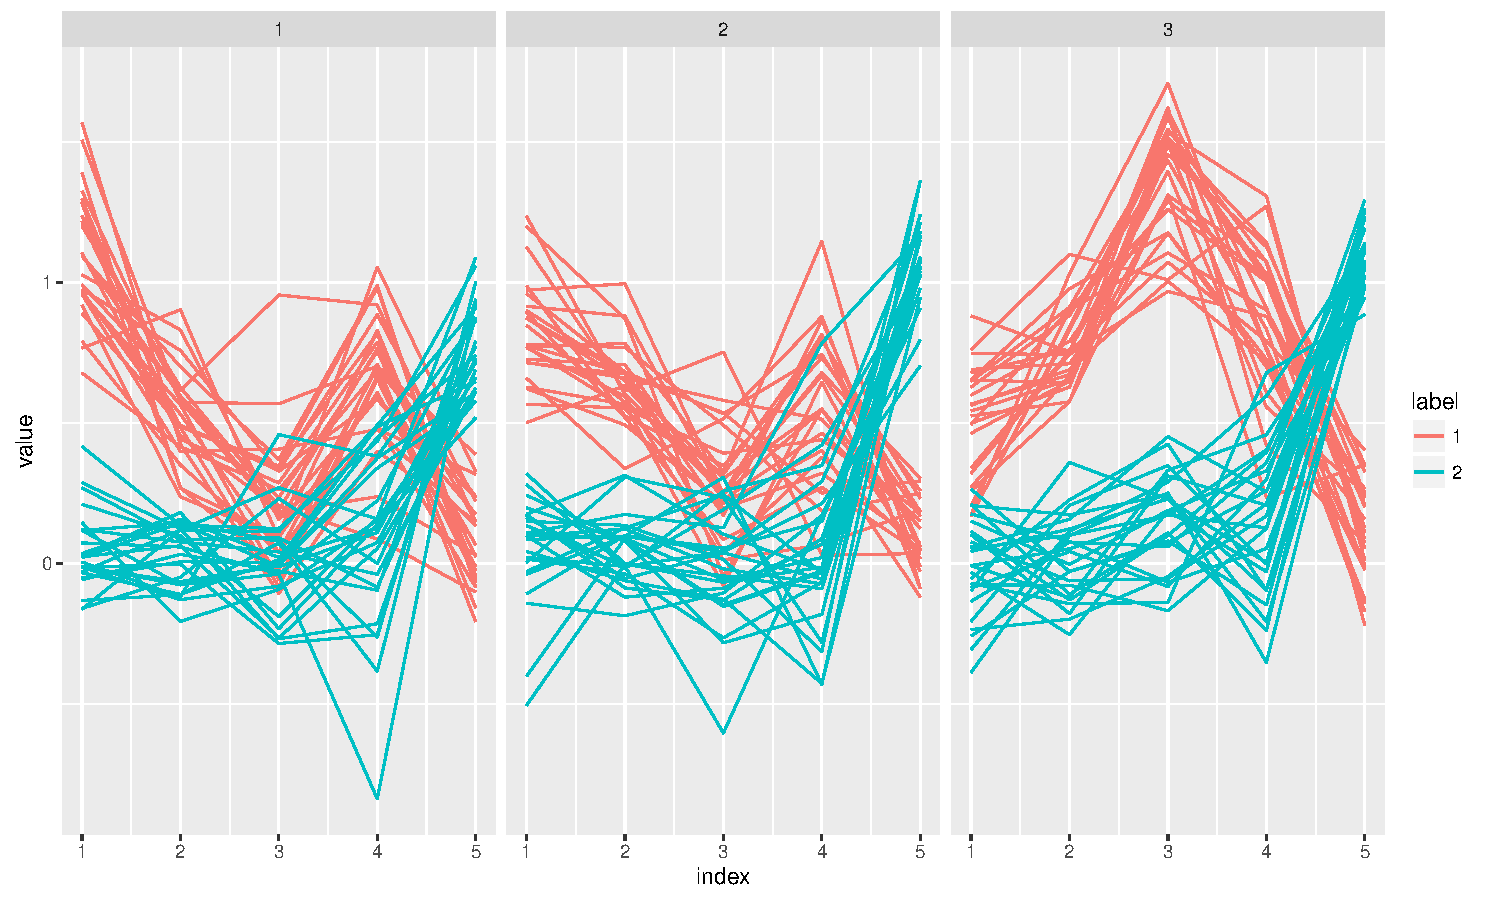
\includegraphics[width=1\columnwidth]{../BatchEffectRemoval/BE_not_removed}
\esfi
\caption{Core estimate with shared factor model.}
\efi

Using the random factor model, the batch effects are captured by the parameters in the random effect factors $f_{j,kr}$, yielding core estimates $c_{ji,r}$ without batch effect while preserving treatment difference.

\bfi
\centering
\bsfi{0.8\columnwidth}
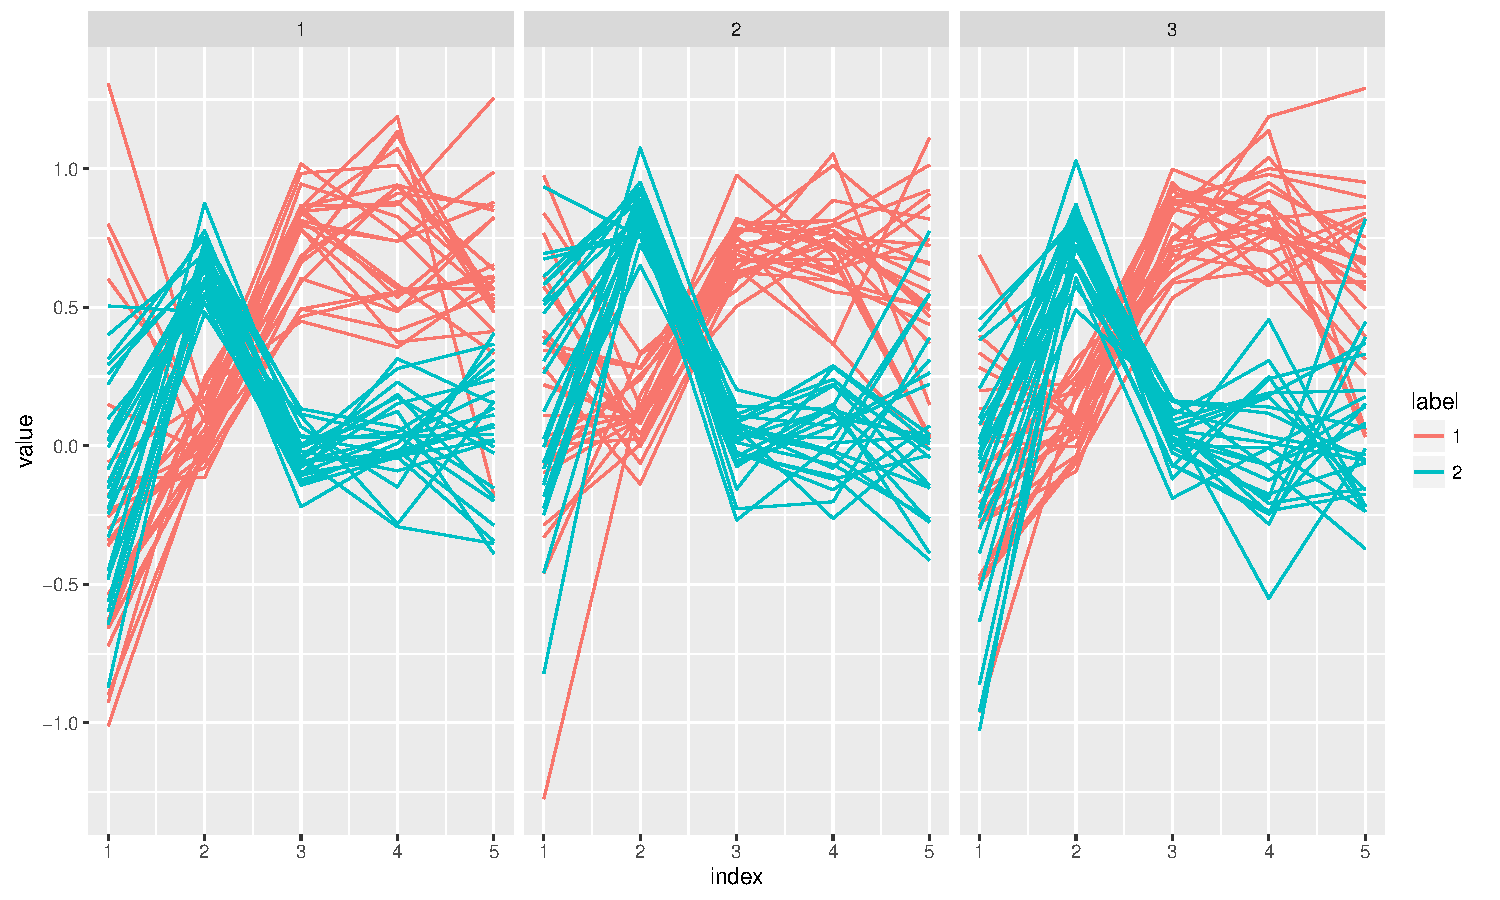
\includegraphics[width=1\columnwidth]{../BatchEffectRemoval/batch_removal}
\esfi
\caption{Core estimate with random factor model.}
\efi


\section{Data Application}

3 datasets:

Sample size:
BNU1: 81
KKI2009: 42
MRN114: 110

\bfi
\centering
\bsfi{0.32\columnwidth}
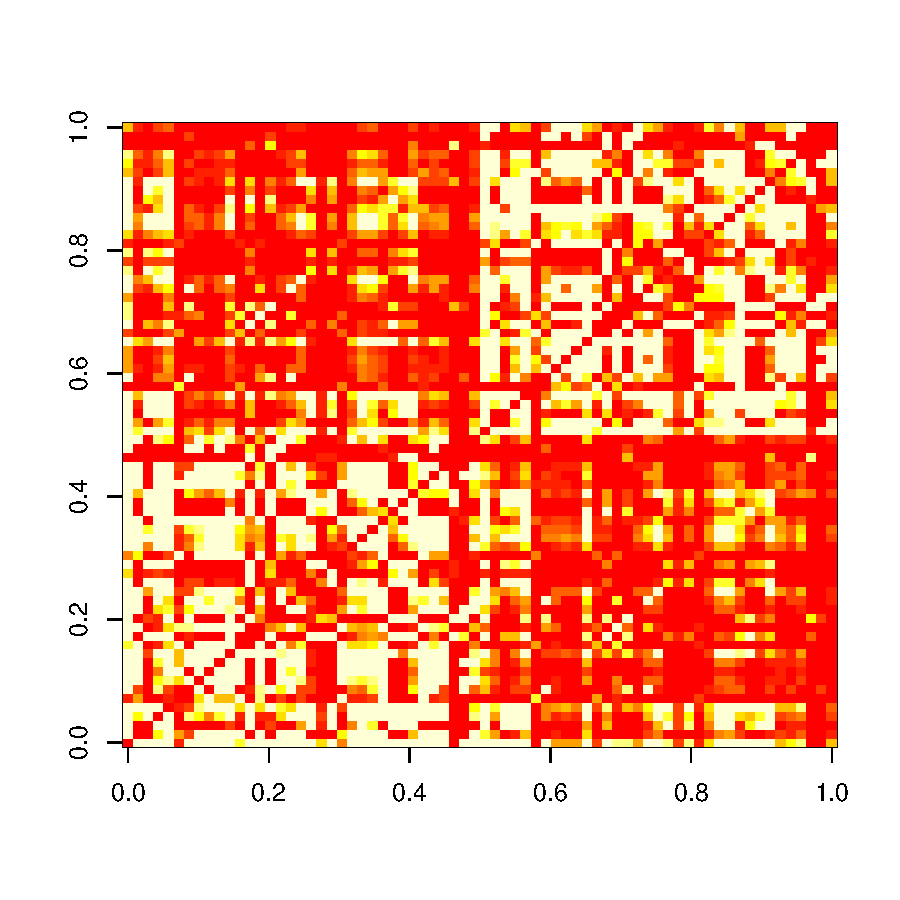
\includegraphics[width=1\columnwidth]{../BatchEffectRemoval/avgA1}
\caption{BNU1}
\esfi
\bsfi{0.32\columnwidth}
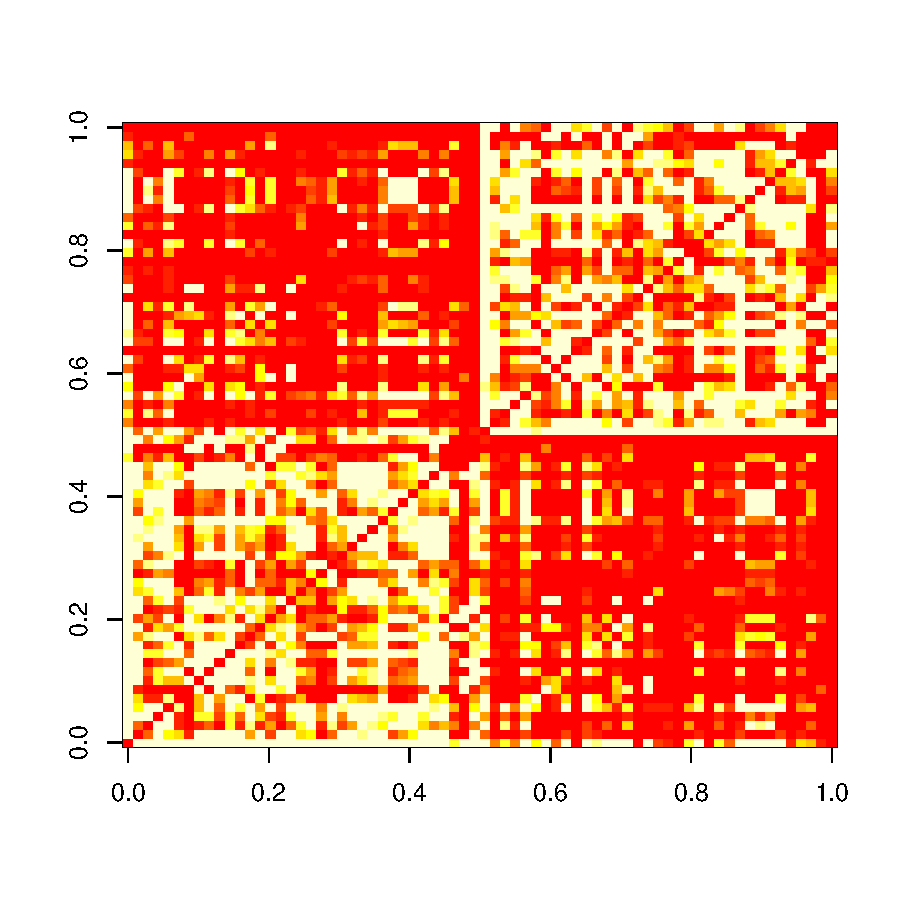
\includegraphics[width=1\columnwidth]{../BatchEffectRemoval/avgA2}
\caption{KKI2009}
\esfi
\bsfi{0.32\columnwidth}
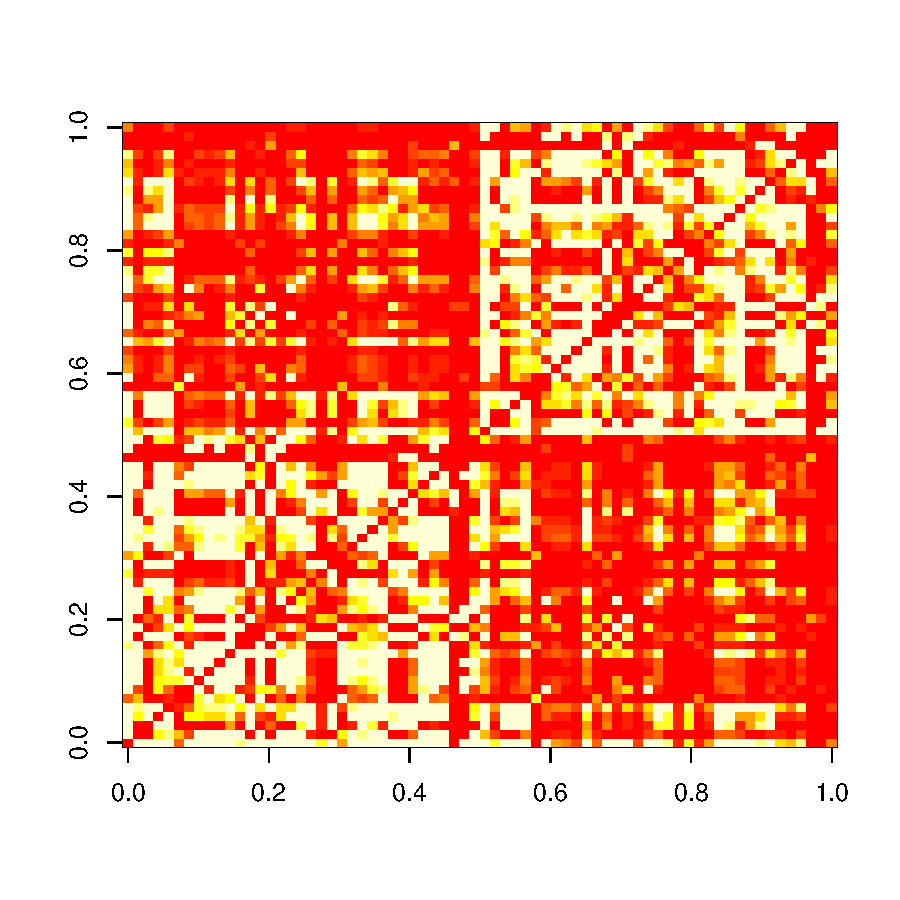
\includegraphics[width=1\columnwidth]{../BatchEffectRemoval/avgA3}
\caption{MRN114}
\esfi

\bsfi{0.32\columnwidth}
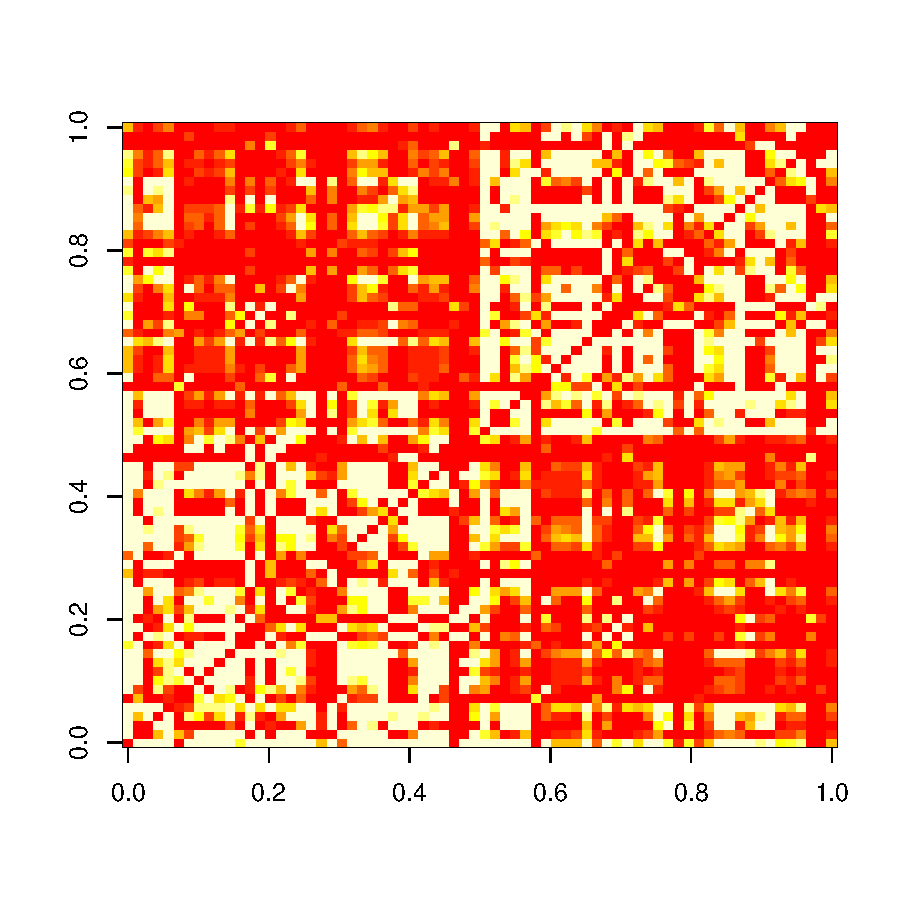
\includegraphics[width=1\columnwidth]{../BatchEffectRemoval/avgA1sex1}
\caption{BNU1, Male}
\esfi
\bsfi{0.32\columnwidth}
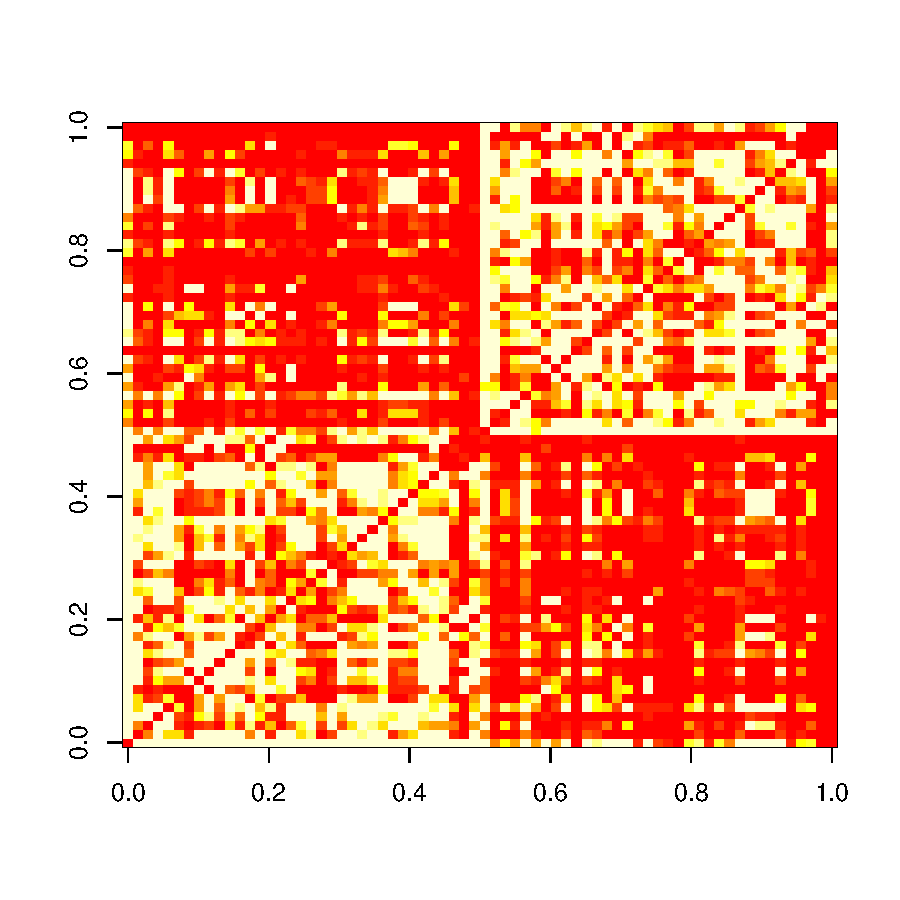
\includegraphics[width=1\columnwidth]{../BatchEffectRemoval/avgA2sex1}
\caption{KKI2009, Male}
\esfi
\bsfi{0.32\columnwidth}
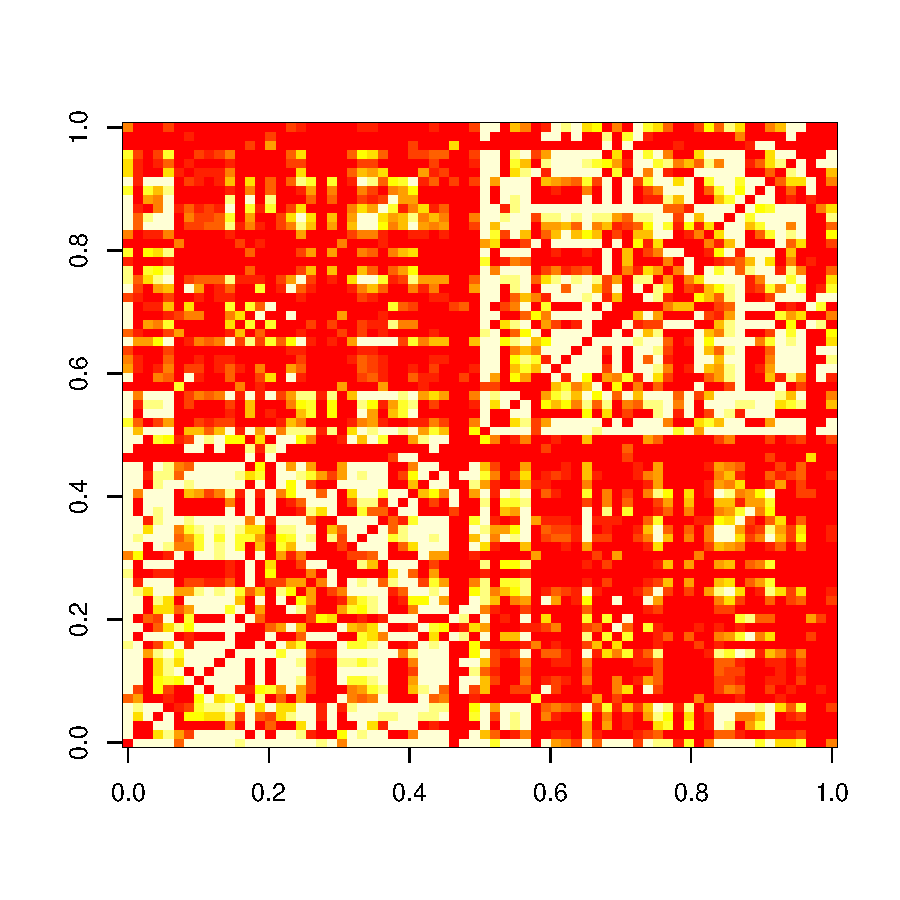
\includegraphics[width=1\columnwidth]{../BatchEffectRemoval/avgA3sex1}
\caption{MRN114, Male}
\esfi

\bsfi{0.32\columnwidth}
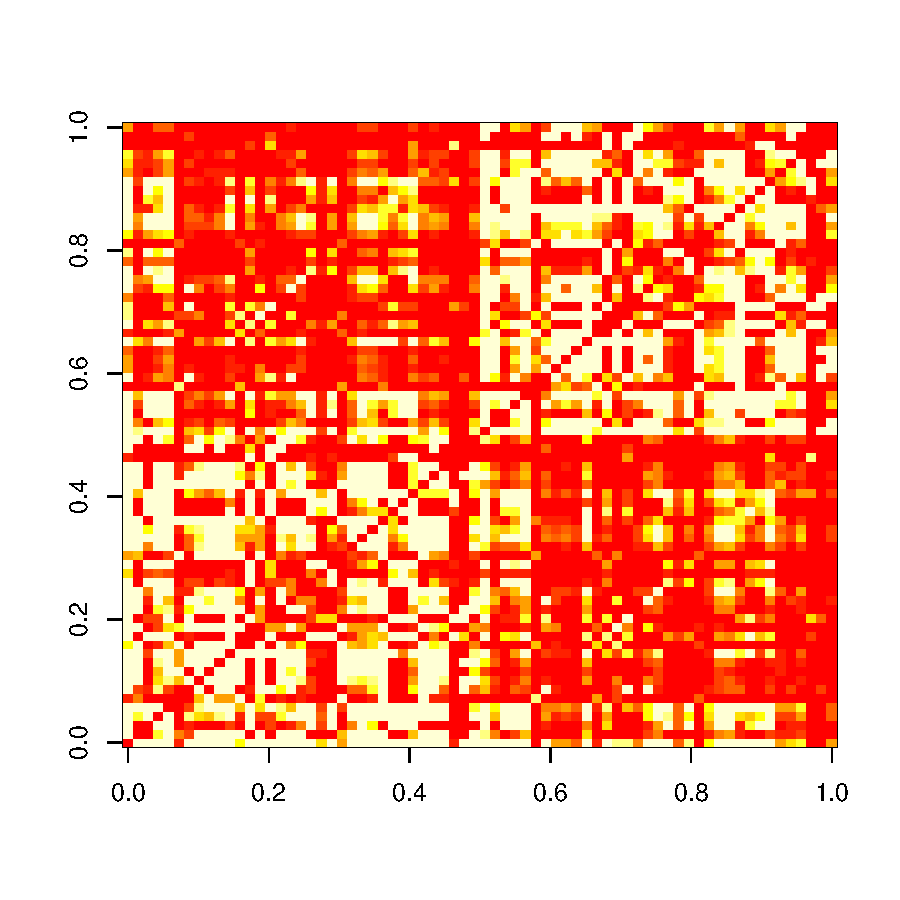
\includegraphics[width=1\columnwidth]{../BatchEffectRemoval/avgA1sex2}
\caption{BNU1, Female}
\esfi
\bsfi{0.32\columnwidth}
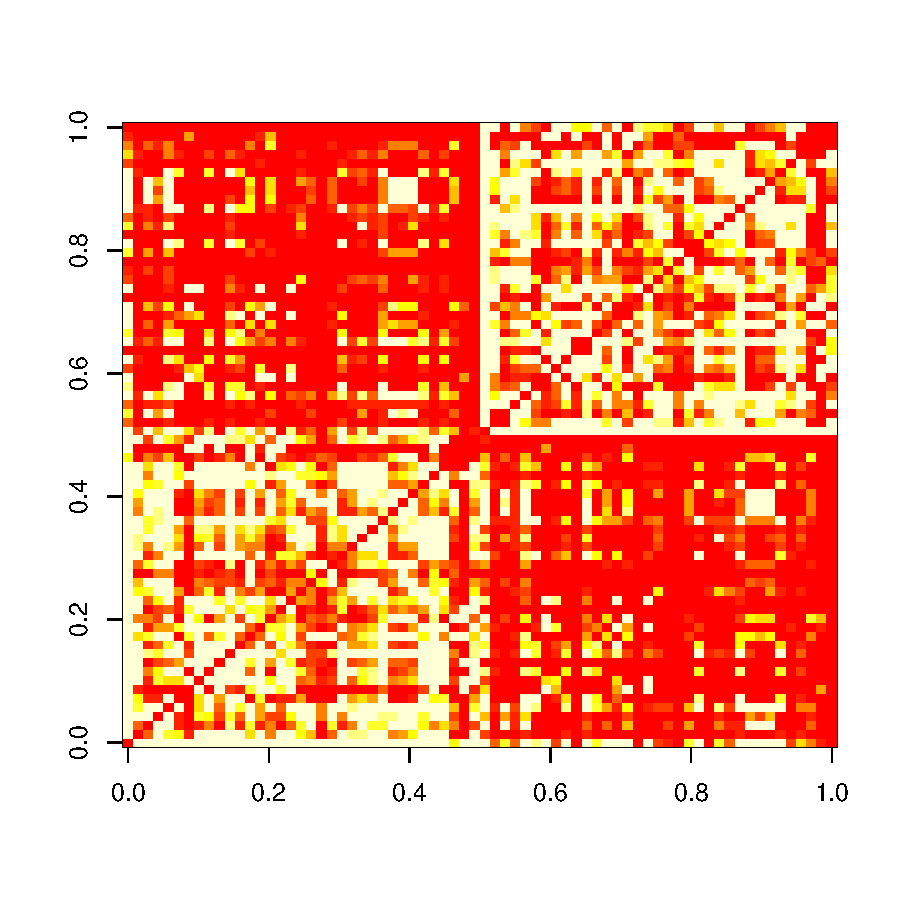
\includegraphics[width=1\columnwidth]{../BatchEffectRemoval/avgA2sex2}
\caption{KKI2009, Female}
\esfi
\bsfi{0.32\columnwidth}
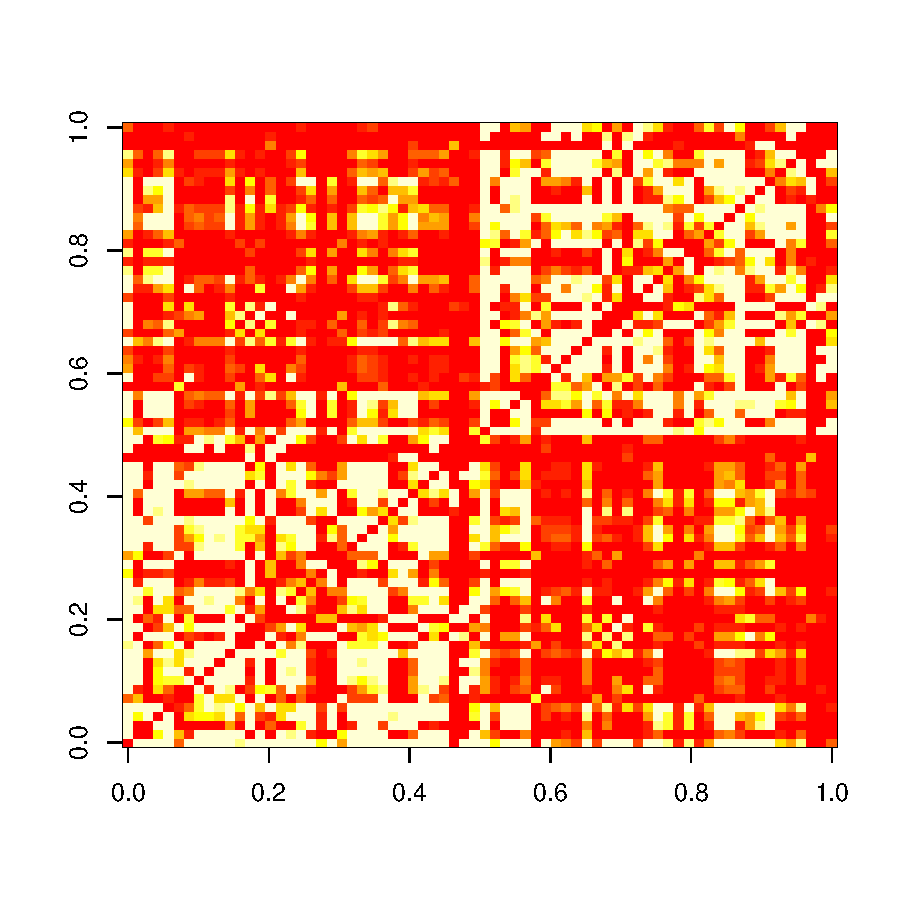
\includegraphics[width=1\columnwidth]{../BatchEffectRemoval/avgA3sex2}
\caption{MRN114, Female}
\esfi
\caption{Group average of the adjacency matrices showing there is a perceptible difference in KKI2009 from BNU1 and MRN114. The difference is in the averages of all subjects, male only and female only.}
\efi

In shared factor model, the between-group variability is passed to the core, leading to confounding of between-treatment difference.


\bfi
\centering
\bsfi{0.8\columnwidth}
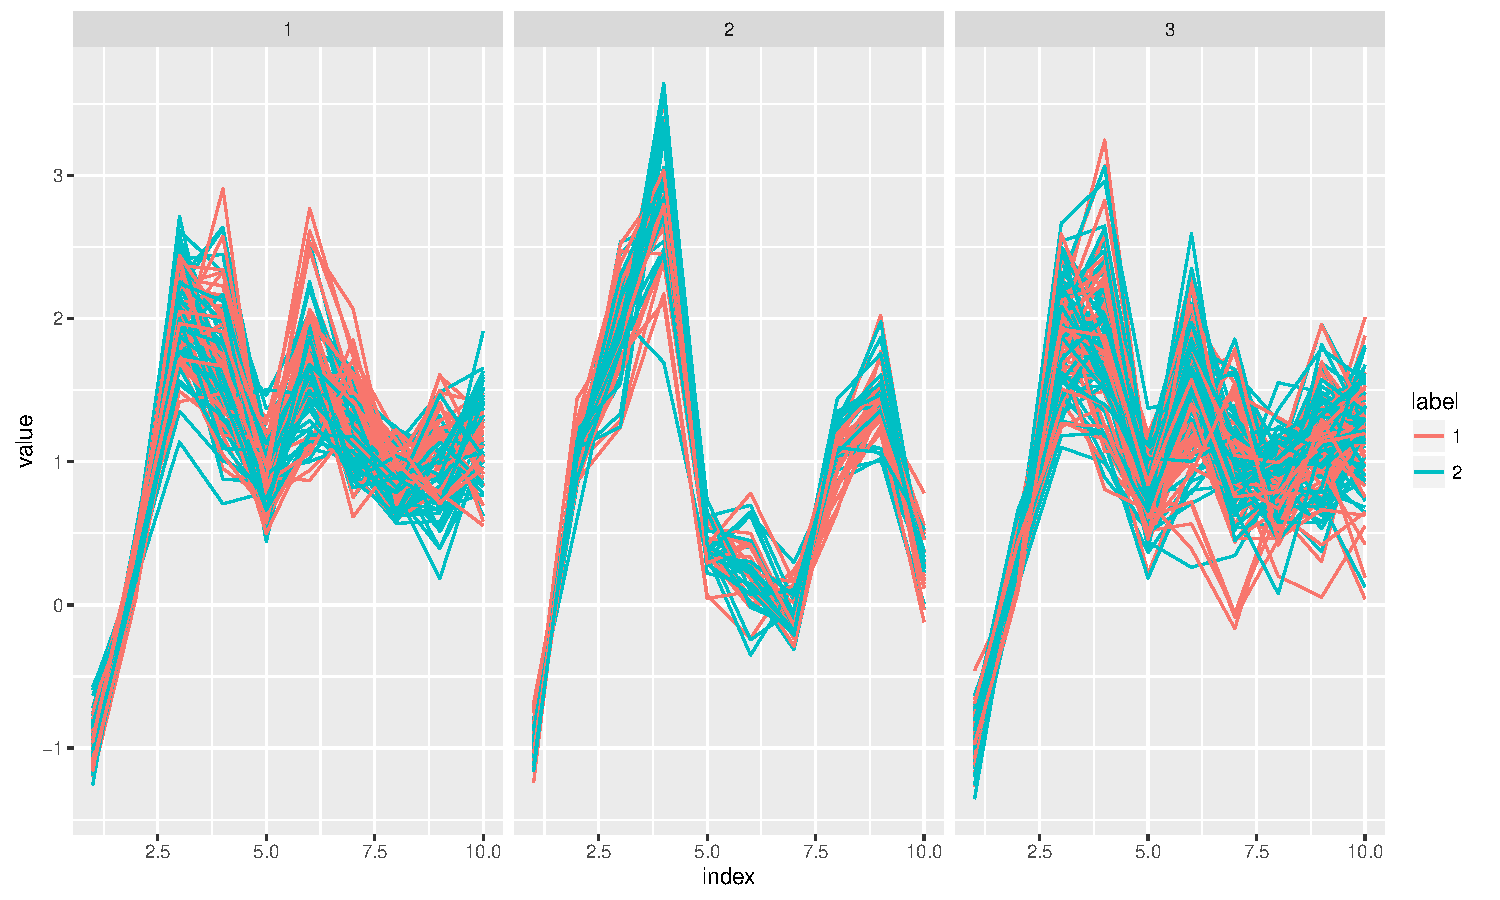
\includegraphics[width=1\columnwidth]{../BatchEffectRemoval/BE_not_removed_data}
\esfi
\caption{Core estimate with shared factor model.}
\efi

\bfi
\centering
\bsfi{0.8\columnwidth}
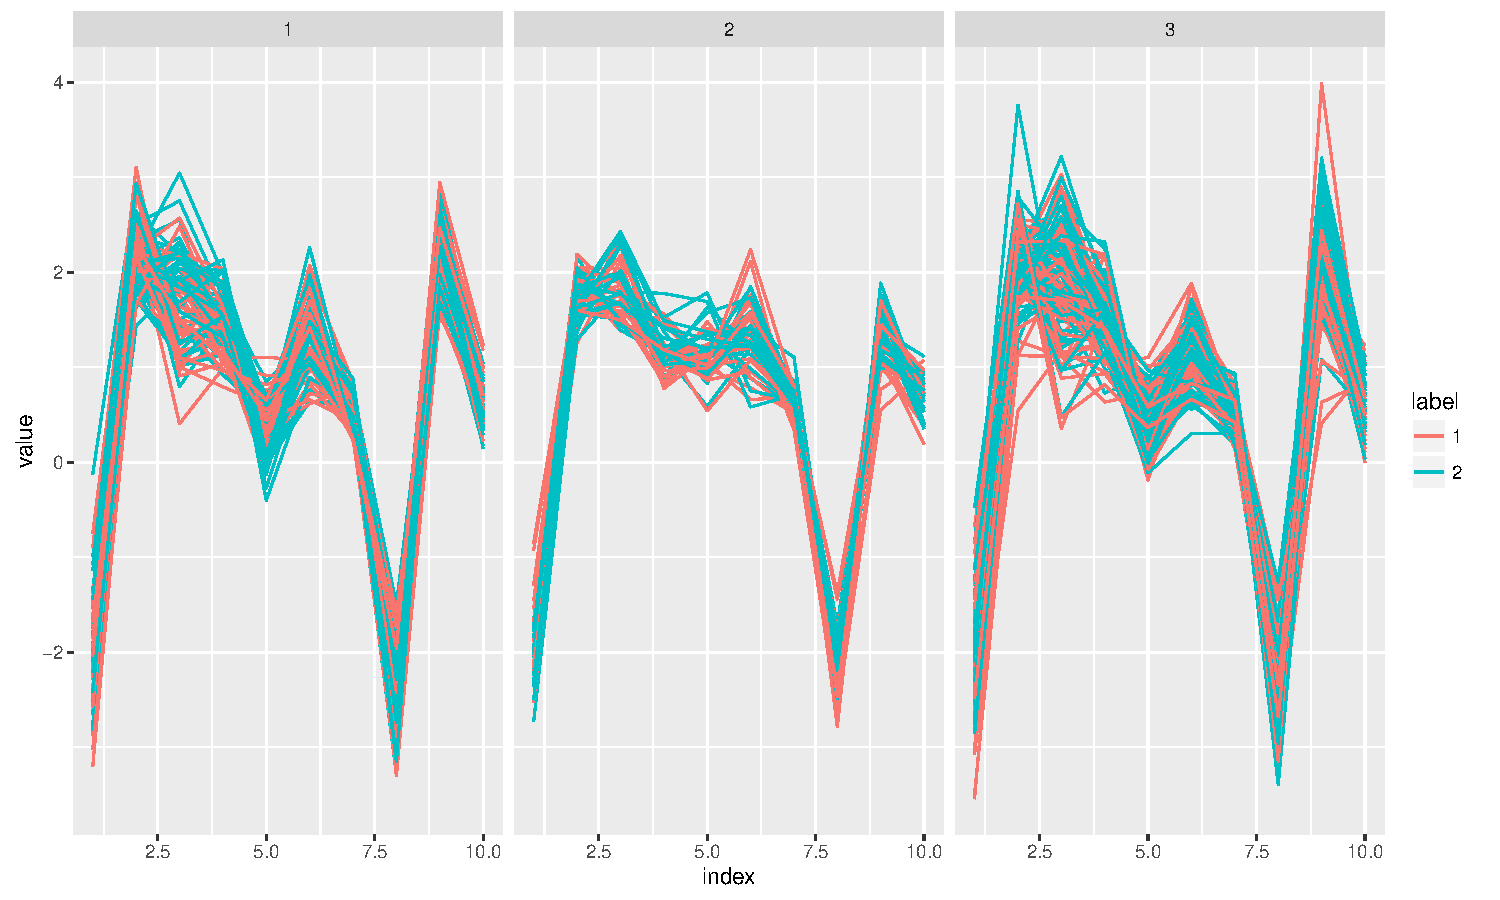
\includegraphics[width=1\columnwidth]{../BatchEffectRemoval/batch_removal_data}
\esfi
\caption{Core estimate with random factor model.}
\efi

Under same rank (d=10), the random factor model has clear better performance than the shared factor model.

\bfi
\centering
\bsfi{0.8\columnwidth}
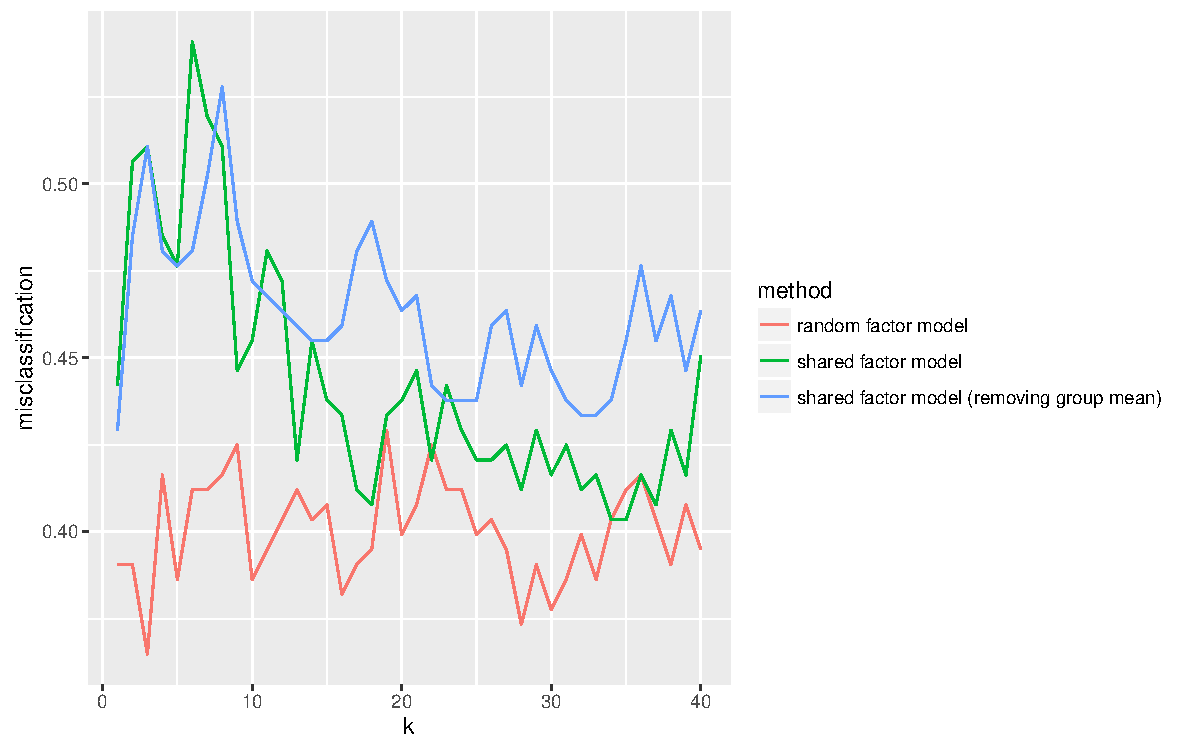
\includegraphics[width=1\columnwidth]{../BatchEffectRemoval/misclassification_data_knn}
\esfi
\caption{K-nearest-neighbor misclassification error shows that the core extracted from tensor factorization with factor random effects having clear better performance in classification.}
\efi

\bibliography{reference}
\bibliographystyle{plainnat}


\end{document}
